%!TEX root = ../main.tex
\chapter{Systembeskrivelse}
Som før nævnt er systemet et automatisk vandingssystem. På figur \ref{photo:RigeBillede} ses et rigebillede af systemet. Systemet tilgås af et grafisk bruger interface som vil være en webside der logges ind på, via en PC. Her gives der mulighed for at se pH-værdi i karet, se hvor meget vand der er i karet samt jordfugtigheden i planterne. Der vil også være mulighed for at indstille disse værdier således systemet selv opretholder dem. Systemet er bestående af en  Raspberry-Pi som kører Raspbian, hvilket er en verision af linux. Systemet kan måle fugtigheden i planterne via en jordfugt-måler der er koblet på I2C bussen. Når fugtigheden når ned under et bestemt niveau tændes der for vandingen. I vandkaret er der iblandet gødning og en korrekt pH-værdi vil blive opretholdt af systemet. Systemet kan måle pH-værdien via en pH-probe som sidder fastmonteret i vandkaret.  
\begin{figure}[H]
	\centering
	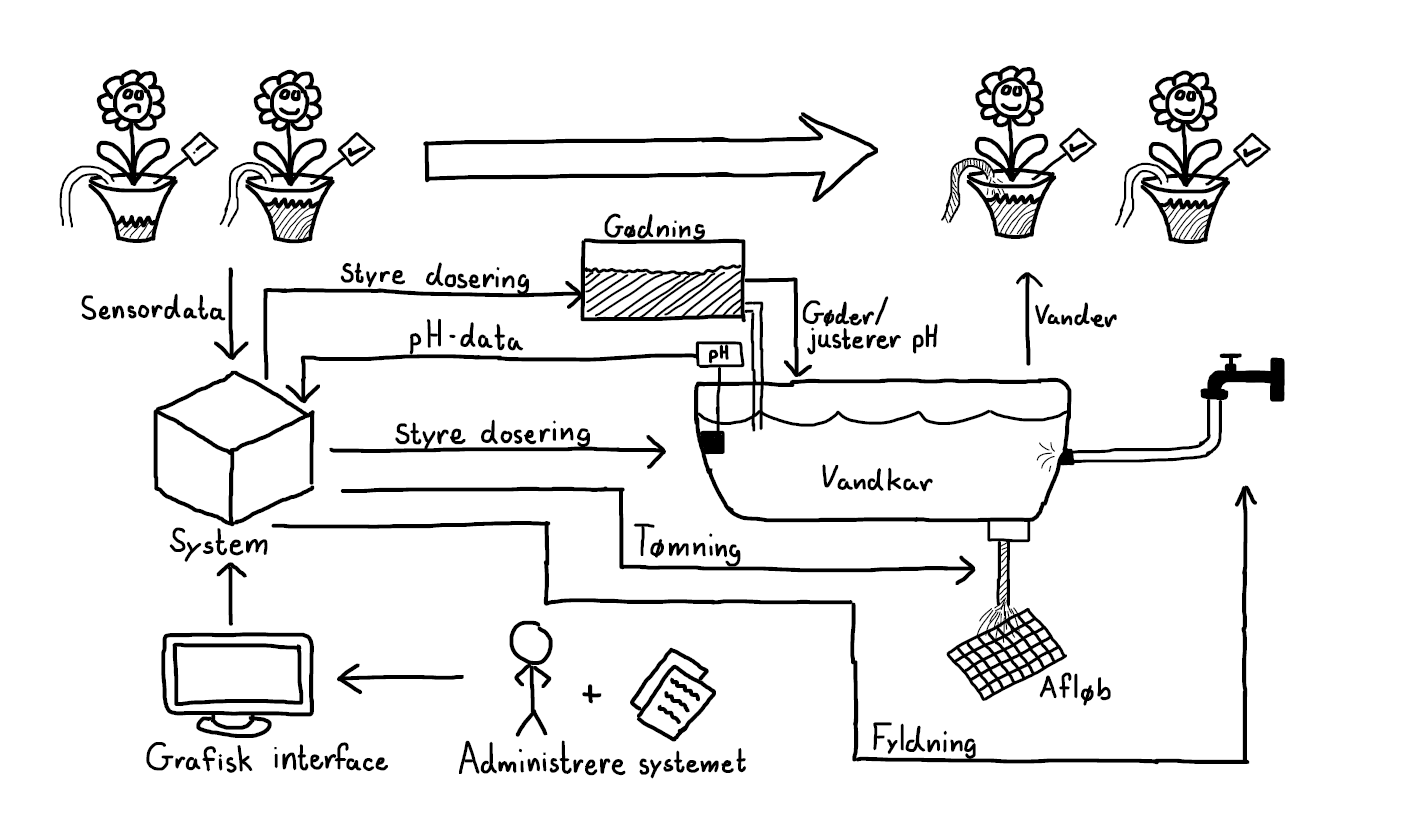
\includegraphics[scale=0.45]{systembeskrivelse/rigebillede}
	\caption{Rigebillede}
	\label{photo:RigeBillede}
\end{figure}
Når systemet startes op vil vandkaret være tomt. For at fylde karet med vand, tændes der for en ventil som sidder direkte på en vandhane. Hermed vil der løbe vand ind i karet og mængden af vand vil blive målt af systemet med en flowmåler. Når der er løbet tilpas mængder vand ind i karet vil ventilen lukke og der vil automatisk blive doseret gødning indtil til en bestemt pH-værdi er nået. Skulle det ske under opfyldning af det ikke lykkedes at lukke indløbsventilen vil der blive åbnet for udløbsventilen. På figur \ref{photo:UseCases} ses de forskellige usecases over systemet.
\begin{figure}[H]
	\centering
	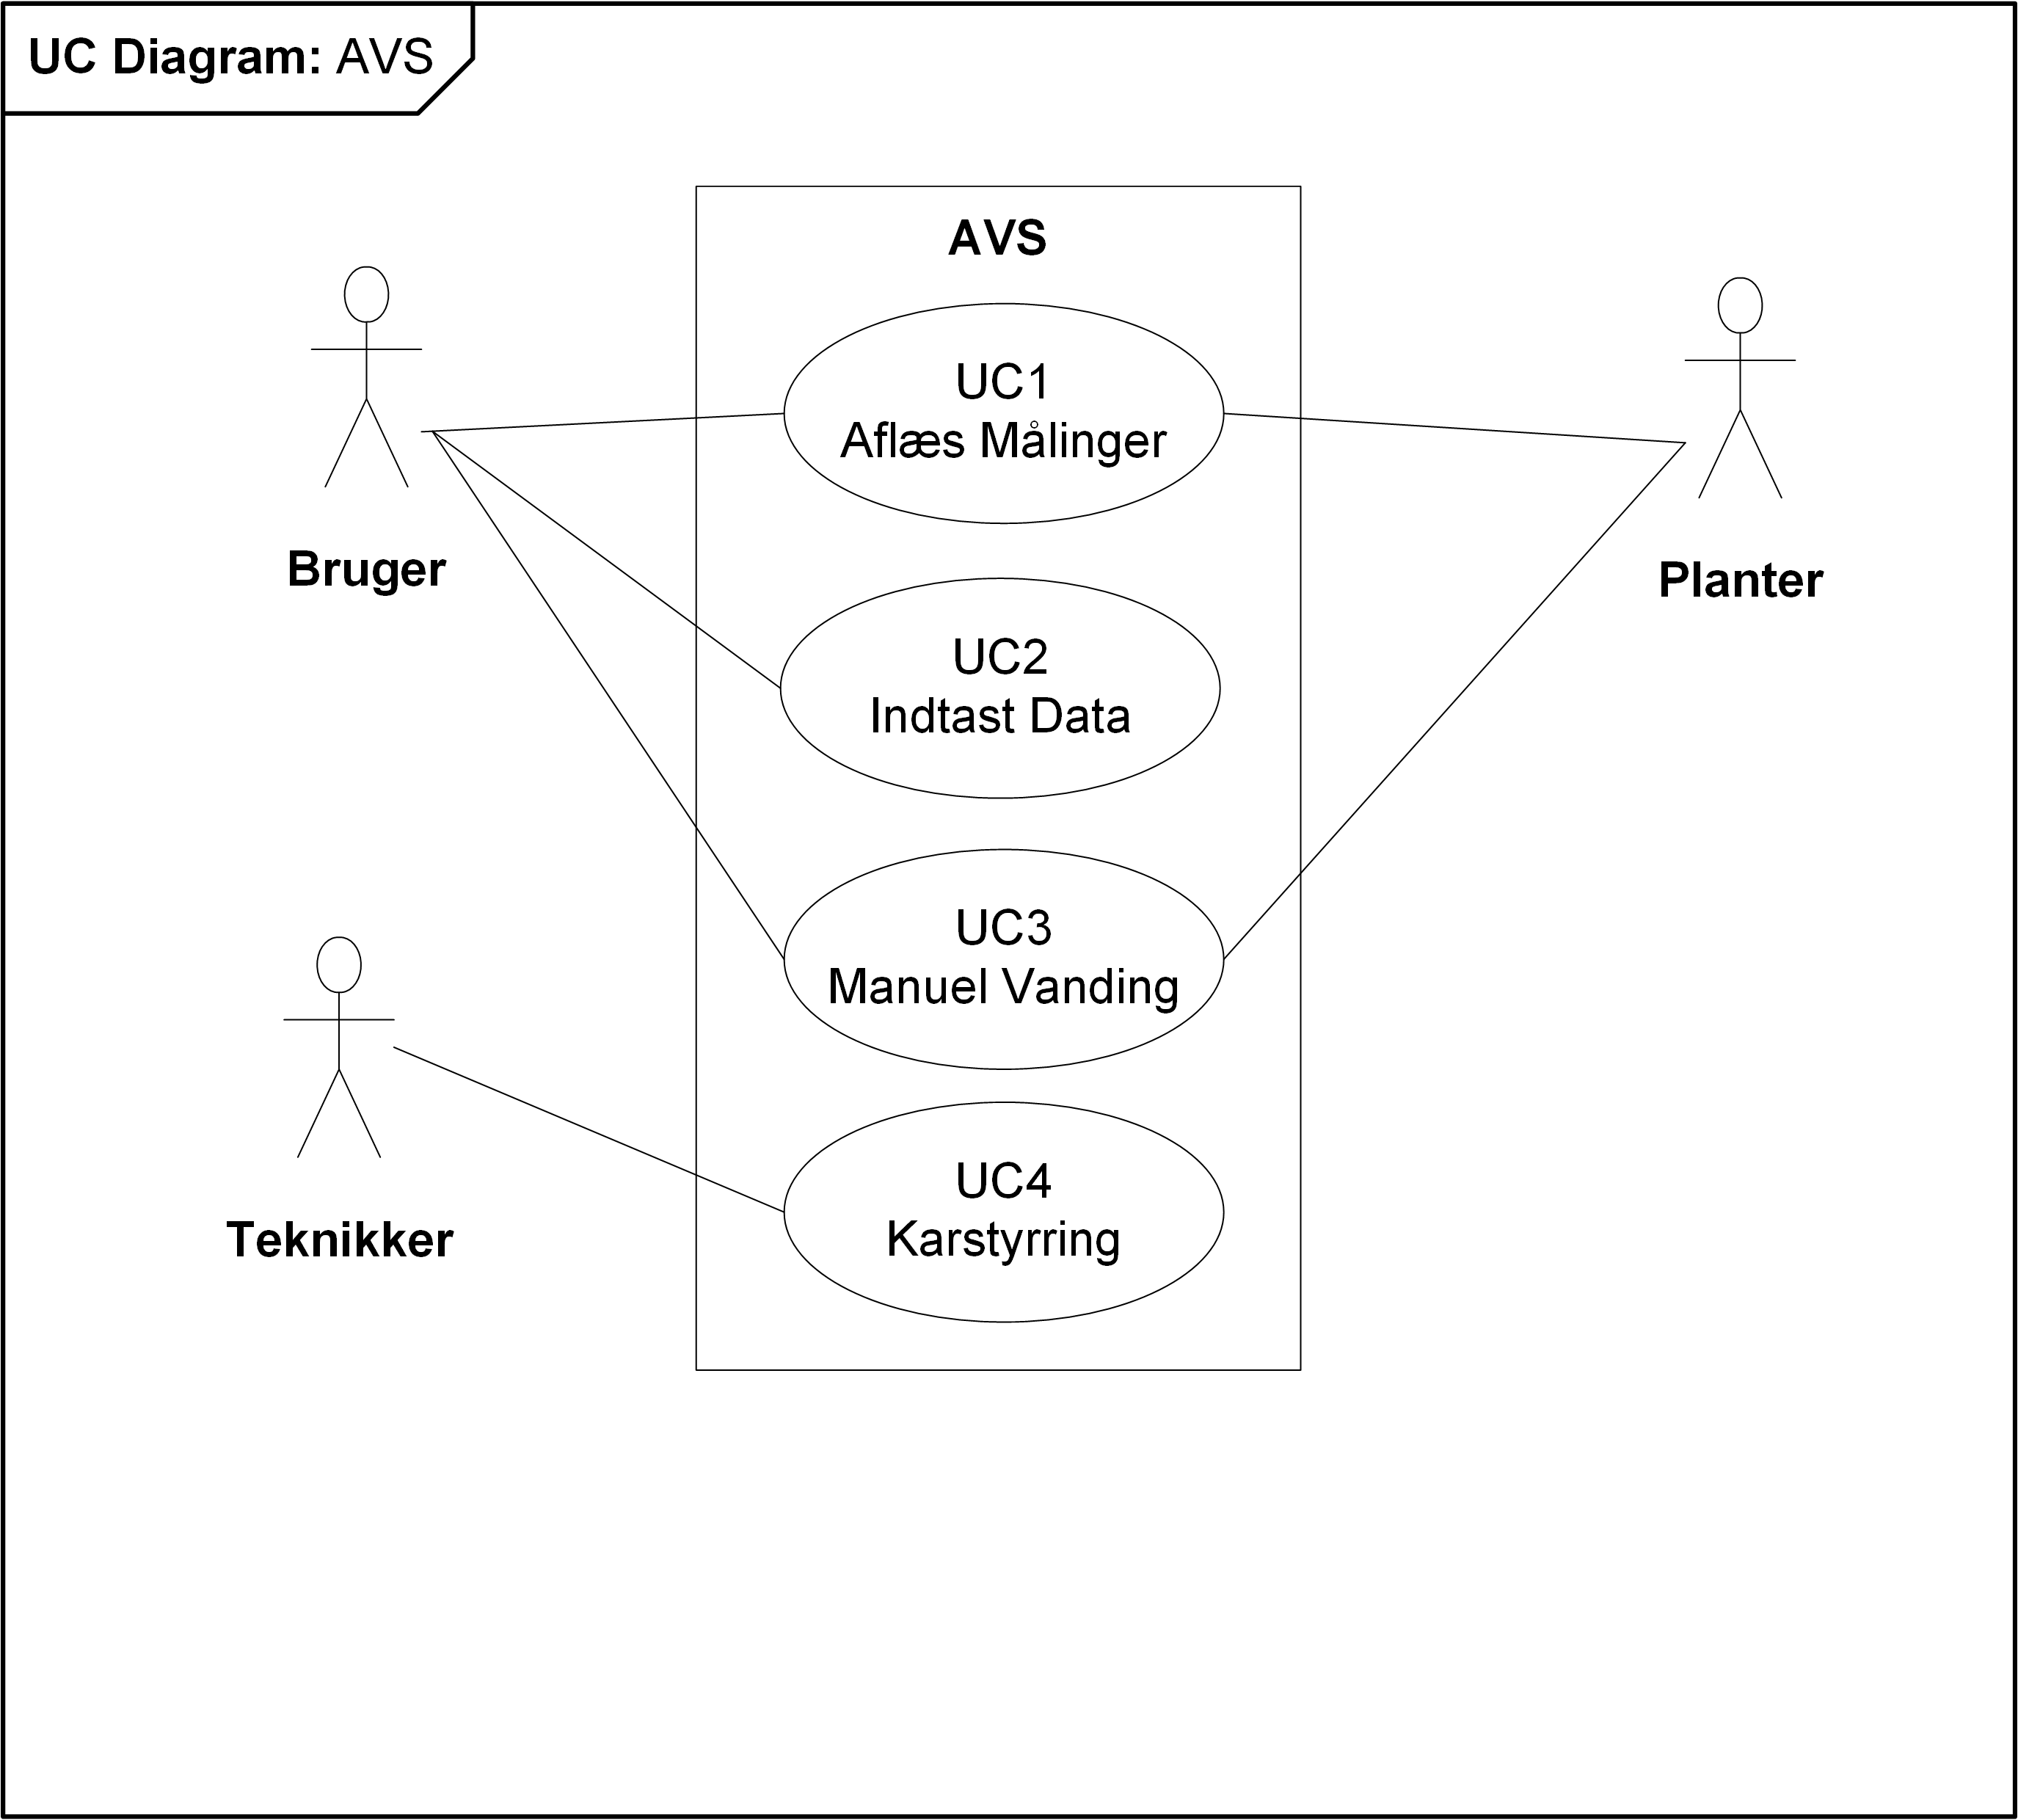
\includegraphics[scale=0.6]{systembeskrivelse/AVS_UseCases}
	\caption{UseCases}
	\label{photo:UseCases}
\end{figure}
Der er to aktører som kan tilgå systemet. Den ene er brugeren som tildaglig bruger systemet. Den anden er teknikeren som tilgår systemet ved oprettelse, vedligeholdelse og nedlæggelse af systemet. Når systemet oprettes bruges usecasen "Opret kar" her opsættes et vandkar og systemet får besked om hvilke sensore der er koblet til via usecasen "Opret Sensor Ø". En sensor Ø er et print som videreformidler dataen fra fx. jordfugtmåleren. Det vil væremuligt at koble flere typer af sensore til fx. en temperatur måler eller flere af samme type. Når karet er oprettet skal pH-proben kalibreres "Kalibrer pH-probe", dette skal gøres en gang hver måned for at kunne sikre en korrekt måling. På selve vandkaret er der en styring som vi kalder for "karprintet" her er pH-proben koblet til. Der vil være en rød LED som lyser på karprintet når pH-proben skal kalibreres. Ved kalibrering sættes proben ned i en buffer-væske som har pH-værdien 7 og der trykkes på en knap på karprintet. Karprintet vil herefter indlæse værdien og den røde LED skifter til en grøn. usecasen "Fyld kar" bruges når karet skal fyldes manuelt. Her gives der mulighed for at åbne indløbsventilen og stoppe den når den ønskede mængde vand er løbet ind. I usecasen "Indtast pH-værdi" gives der mulighed for at indtaste en pH-værdi som systemet skal tilnærme. Det samme gives der mulighed for i "Indtast volumen". I usecasen "Aflæs målinger" går brugeren ind og aflæser værdierne fra sensorerne hvis det ønskes at se hvad statussen er. Usecasen "Manuel vanding" giver mulighed for at vande manuelt. Dette kan være ønskeligt hvis systemet har fejl ved sensorene. Usecasen "Tøm kar" bruges til at tømme karet og "Slet kar" er for at nedlægge et oprettet kar.  